\section{GEO-Cloud Graphical User Interface}
\label{sec:interfaz}
In this section, the \ac{GUI} developed for managing the execution of the defined
scenarios in GEO-Cloud experiment is exposed. First, the architecture is
explained. The components of the graphical user interface are described. Then, the interface is shown to identify the components.

\subsection{Architecture}

The graphical user interface of GEO-Cloud experiment is composed by the following classes:

\begin{itemize}

\item \emph{Experiment Controller}: it manages the \sss turning on or shutting it down by using \ac{SSH} connections and it obtains the workload of the \emph{Orchestrator} and \emph{Processing Chain} machine.
\item \emph{SSH Connection}: it creates an \emph{SSH} connection with a \vw machine.
\item \emph{SSH Order}: it remotely executes an  \emph{SSH} order in a \emph{SSH Connection}.
\item \emph{getLoad}: it obtains the workload of the \emph{Orchestrator} and \emph{Processing Chain} machines.
\item \emph{JFedParser}: it parsers the \emph{Rspec} obtained from the \emph{JFed} software once the \vw deployment was made to obtain the hostnames of the \vw nodes.
\item \emph{UI Controller}: it manages the graphical widgets and the \emph{Experiment Controller} interactions.
\item \emph{Video Widget}: it shows a video demonstration of the satellite constellation acquiring images at same time that the satellites do it in \vw.
\item \emph{About Widget}: it shows the \emph{About} window where the acknowledments are shown.
\item \emph{Log Widget}: it prints the logs which receives from satellites and ground stations.
\item \emph{Tab Widget}: it contains two graphics to plot the workload of the \emph{Orchestrator} and the \emph{Processing Chain} machines.
\end{itemize}

The Figure~\ref{fig:gui-class} shows the class diagram where the relations between the components are pictured.

\begin{figure}[!h]
\begin{center}
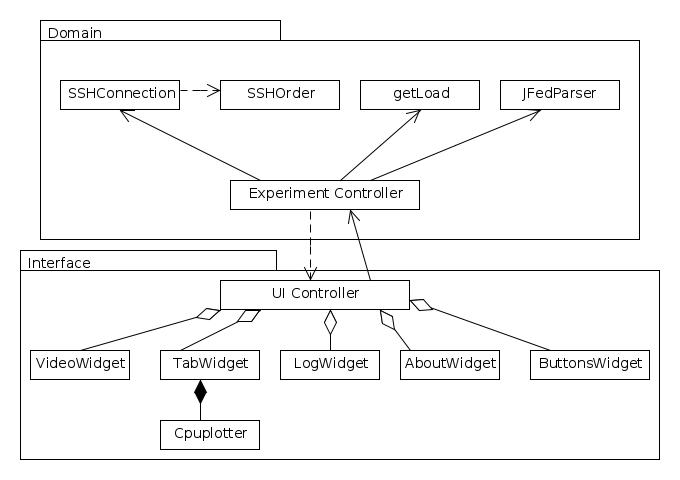
\includegraphics[width=0.7\textwidth]{gui/gui-class.jpg}
\caption{Class diagram of the graphical user interface}
\label{fig:gui-class}
\end{center}
\end{figure}


\subsubsection{Experiment Controller}

The functions of the \emph{Experiment Controller} are the following:
\begin{itemize}
\item To obtain the hostnames of the \vw nodes included in the \emph{Rspec} file located in ``source/gui/resources/jfed.out''. It creates a \emph{JFedParser} object to do this. These hostnames are used to create \emph{SSH Connections} objects to send orders to the \vw nodes.
\item To create the \emph{SSH Connections} of all the nodes deployed in \vw.
\item To create the \emph{SSH Commands} to manage the experimentation in \vw.
\item To obtain the workload of both the \emph{Orchestrator} and \emph{Processing Chain} machines. Then, these measures are sent to the \emph{UI Controller} for plotting.
\item To communicate the experiment logs from \vw to the \emph{UI Controller}.
\end{itemize}

\paragraph{Experiment Controller Workflow}~\\

The workflow of the \emph{Experiment Controller} is the following:
\begin{enumerate}
\item The file which contains the \emph{Rspec} is parsed.
\item Using the hostnames obtained, it creates a \emph{SSH Connection} per hostname obtained.
\item When the experimenter selects an scenario and pushes the start button, the \emph{Experiment Controller} creates \emph{SSH Commands} indicating to start the selected scenario and sends to \vw nodes by using the \emph{SSH Connection} objects. Moreover, it starts the reproduction of the video of the selected scenario.
\item When the experimenter selects an scenario and pushes the stop button, the \emph{Experiment Controller} creates \emph{SSH Commands} indicating to stop the selected scenario and sends to \vw nodes by using the \emph{SSH Connection} objects.
\item The log from the \emph{SSH Commands} performed is collected and it sends them to the \emph{UI Controller}.
\item Two \emph{getLoad} objects are created to connect with the \emph{Orchestrator} and the \emph{Processing Chain} machines to obtain in real time their workload by using \emph{SSH Connections}. The workloads are passed to the \emph{UI Controller} for plotting.
\end{enumerate}

\subsubsection{SSH Connection}

This class connects through the \emph{Virtuall Wall Bastion} machine to the \vw nodes. This connection is performed by using the public key obtained in Section~\ref{sec:first-steps}.

This class has the \emph{executeCommand} method in order to remotely carry out the commands given by the \emph{Experiment Controller}

\paragraph{SSH Connection Workflow}~\\

The workflow of the \emph{SSH Connection} is the following:
\begin{enumerate}
\item The object is created by passing as arguments: the hostname of the \vw machine to connect and the \ac{IP} address of the \vw \emph{Bastion} machine.
\item By using \emph{Paramiko} library, the connection is performed.
\item When a command is executed, the log is returned and sended to the \emph{Experiment Controller} class.
\end{enumerate}


\subsubsection{SSH Order}

This class creates a \emph{SSH order} to send it through a \emph{SSH Connection} object.

\paragraph{SSH Connection Workflow}~\\

The workflow of the \emph{SSH Connection} is the following:
\begin{enumerate}
\item The object is created by passing as argument the order to remotely be executed.
\end{enumerate}

\subsubsection{getLoad}

This class obtains the  workload of the both \emph{Orchestrator} and  \emph{Processing Chain} machines by using a \emph{SSH Command} through their \emph{SSH Connections} objects.

\paragraph{getLoad Workflow}~\\

The workflow of the \emph{getLoad} is the following:
\begin{enumerate}
\item The object is created by passing as argument the \ac{IP} address of remote machine.
\item A \emph{SSH Connection} to machine is created.
\item Periodically, it sends a \emph{SSH Order} to get the workload though the \emph{SSH Connection}.
\end{enumerate}

\subsubsection{JFedParser}

This class parser the  \emph{Rspec} of the \emph{JFed} to obtain the hostnames of the \vw nodes.

\paragraph{JFedParser Workflow}~\\

The workflow of the \emph{JFedParser} is the following:
\begin{enumerate}
\item The object is created by passing as argument the path of the \emph{Rspec} file.
\item By using a \ac{XML} Python parser (Minidom library) obtains the hostnames of all nodes deployed in \vw.
\item When the operation \emph{getHostnames} is called, the hostnames are returned.
\end{enumerate}

\subsubsection{UI Controller}

The \emph{UI Controller} is based in the \emph{Controller} design pattern and it has the following functionalities:
\begin{itemize}
\item To manage the experiment status through graphical widget interactions and sends them to the \emph{Experiment Controller}.
\item To show the experiment status such as the workload, logs and video from \emph{Experiment Controller}.
\end{itemize}

\paragraph{UI Controller Workflow}~\\

The workflow of the \emph{UI Controller} is the following:
\begin{enumerate}
\item It commands to the \emph{Experiment Controller} to execute the experiment when the user selects an scenario and  it and clicks the start button. When the users starts the execution, the video of the selected scenario is started by calling to the \emph{Video Widget} with the selected scenario.
\item  It commands to the \emph{Experiment Controller} to stop the execution of the experiment when the user clicks the stop button
\item It receives the logs from the \emph{Experiment Controller} and sends to the \emph{Log Widget} to show them.
\item It receives the workloads from the \emph{Experiment Controller} and sends to the \emph{Tab Widget} to plot them.
\item When the user pushes the \emph{About Button}, the \emph{About Widget} is created and shown.
\end{enumerate}

\subsubsection{Video Widget}

This class reproduces the video corresponding of the selected scenario. 

\paragraph{Video Widget Workflow}~\\

The workflow of the \emph{Video Widget} class is the following:
\begin{enumerate}
\item When a scenario is started, the \emph{Video Widget} is set up to reproduce the video of the selected scenario.\item When the video finishes, it stops the reproduction.
\end{enumerate}


\subsection{About Widget}
This class shows a dialog with the acknowledments. 

\paragraph{About Widget  Workflow}~\\

The workflow of the \emph{About Widget} class is the following:
\begin{enumerate}
\item When this object is created, it loads the resource images and the ackowledments and shows them.
\end{enumerate}

\subsection{Log Widget}

This class shows the logs received from the \emph{UI Controller}. 

\paragraph{Log Widget  Workflow}~\\

The workflow of the \emph{Log Widget} class is the following:
\begin{enumerate}
\item When the \emph{UI Controller} calls the \emph{appendLog} operation of the \emph{Log Widget}, the logs sent as parameter are shown in the \ac{GUI}.
\end{enumerate}

\subsection{Tab Widget}

This class has two \emph{CPUPlotter} objects. The first one plots the \emph{Orchestrator} workload and the second one, the \emph{Processing Chain} workload. Each one of them are located in a tab in which ones the user can see the workload of the both machines simply changing between them.
The \emph{CPUPlotter} class were carryied out by using the \emph{QWT} libraries of the \emph{QT} framework. It creates a linear plot which changes with the input of new data. It were distributed with \emph{Psymon} application (it was developed by Dimitris Diamantis) under the \ac{GPL}v3 and it was reused in this project.

\paragraph{Tab Widget  Workflow}~\\

The workflow of the \emph{Log Widget} class is the following:
\begin{enumerate}
\item The \emph{UI Controller} sends the workload from the \emph{Experiment Controller} to the \emph{Tab Widget} object. 
\item Depending of the source of the data (\emph{Orchestrator} or \emph{Processing Chain} machine) the data is plotted in one or the other.
\end{enumerate}


\subsection{Implementation of the Graphical User Interface}


The implementation of this module was done in Python 2.7. The python's libraries
needed to implement the software are listed in
Table~\ref{table:gui-libraries}.

\begin{table}[!h]
  \centering
  {\small
  


\begin{tabular}{p{.2\textwidth}p{.2\textwidth}}
  \tabheadformat
  \tabhead{Python Library}   &
  \tabhead{Function}\\
\hline
\textit{Threading}         & System library for creating, syncronizing and managing threads \\
\hline
\textit{OS}         & Library which provides operative system interactions \\
\hline
\textit{Time}         & Libraty to manage the time\\
\hline
\textit{Paramiko}         & Library to create and manage \ac{SSH} connections\\
\hline
\textit{Phonon}         & Library to manage multimedia files and widgets\\
\hline
\textit{Pdb}         &  Used for debugging the software\\
\hline
\textit{PyQT}         &Library used to build the \ac{GUI}  \\
\hline
\textit{Psutil}         &Library used to obtain the workload of the CPU\\
\hline
\textit{XML DOM}         &Library to parse \ac{XML} files\\
\hline
\end{tabular}


% Local variables:
%   coding: utf-8
%   ispell-local-dictionary: "castellano8"
%   TeX-master: "main.tex"
% End:

  }
  \caption{GUI Python Libraries}
  \label{table:gui-libraries}
\end{table}

\subsection{Execution of the Graphical User Interface}

To execute the \ac{GUI} the following dependencies are required:
\begin{itemize}
\item The libraries listed in Table~\ref{table:gui-libraries}. 
\item The last \emph{Rspec} specification of the \vw deployment in \emph{JFed}. This file is located in ``source/gui/resources/jfed.out''.
\item \emph Ethernet interface for the network connection in the \bonfire
  \emph{WAN}.
\item \emph Ethernet interface for connecting with the \vw nodes through the \vw \emph{Bastion}.
\end{itemize}

The execution of the \ac{GUI} is done as follows (the experimenter must be located in ``source/gui'' folder):
\begin{itemize}
\item[>] python main.py
\end{itemize}

\subsection{Components of the Graphical User Interface}

The \acl{GUI} is composed by four well diferenciated elements:
\begin{itemize}
\item \emph{Video zone}: it is the zone where the video of each scenario is reproduced.
\item \emph{Log zone}: it is the zone where the logs are shown during the experiment.
\item \emph{Workload zone}: it is the zone where the workloads of the \emph{Orchestrator} and the \emph{Processing Chain} machines are shown.
\item \emph{User interaction zone}: it is the zone where the experimenter selects the scenario and manages the experiment.
\end{itemize}

The Figure~\ref{fig:gui-components} shows the different components of the graphical user interface.
\begin{figure}[!h]
\begin{center}
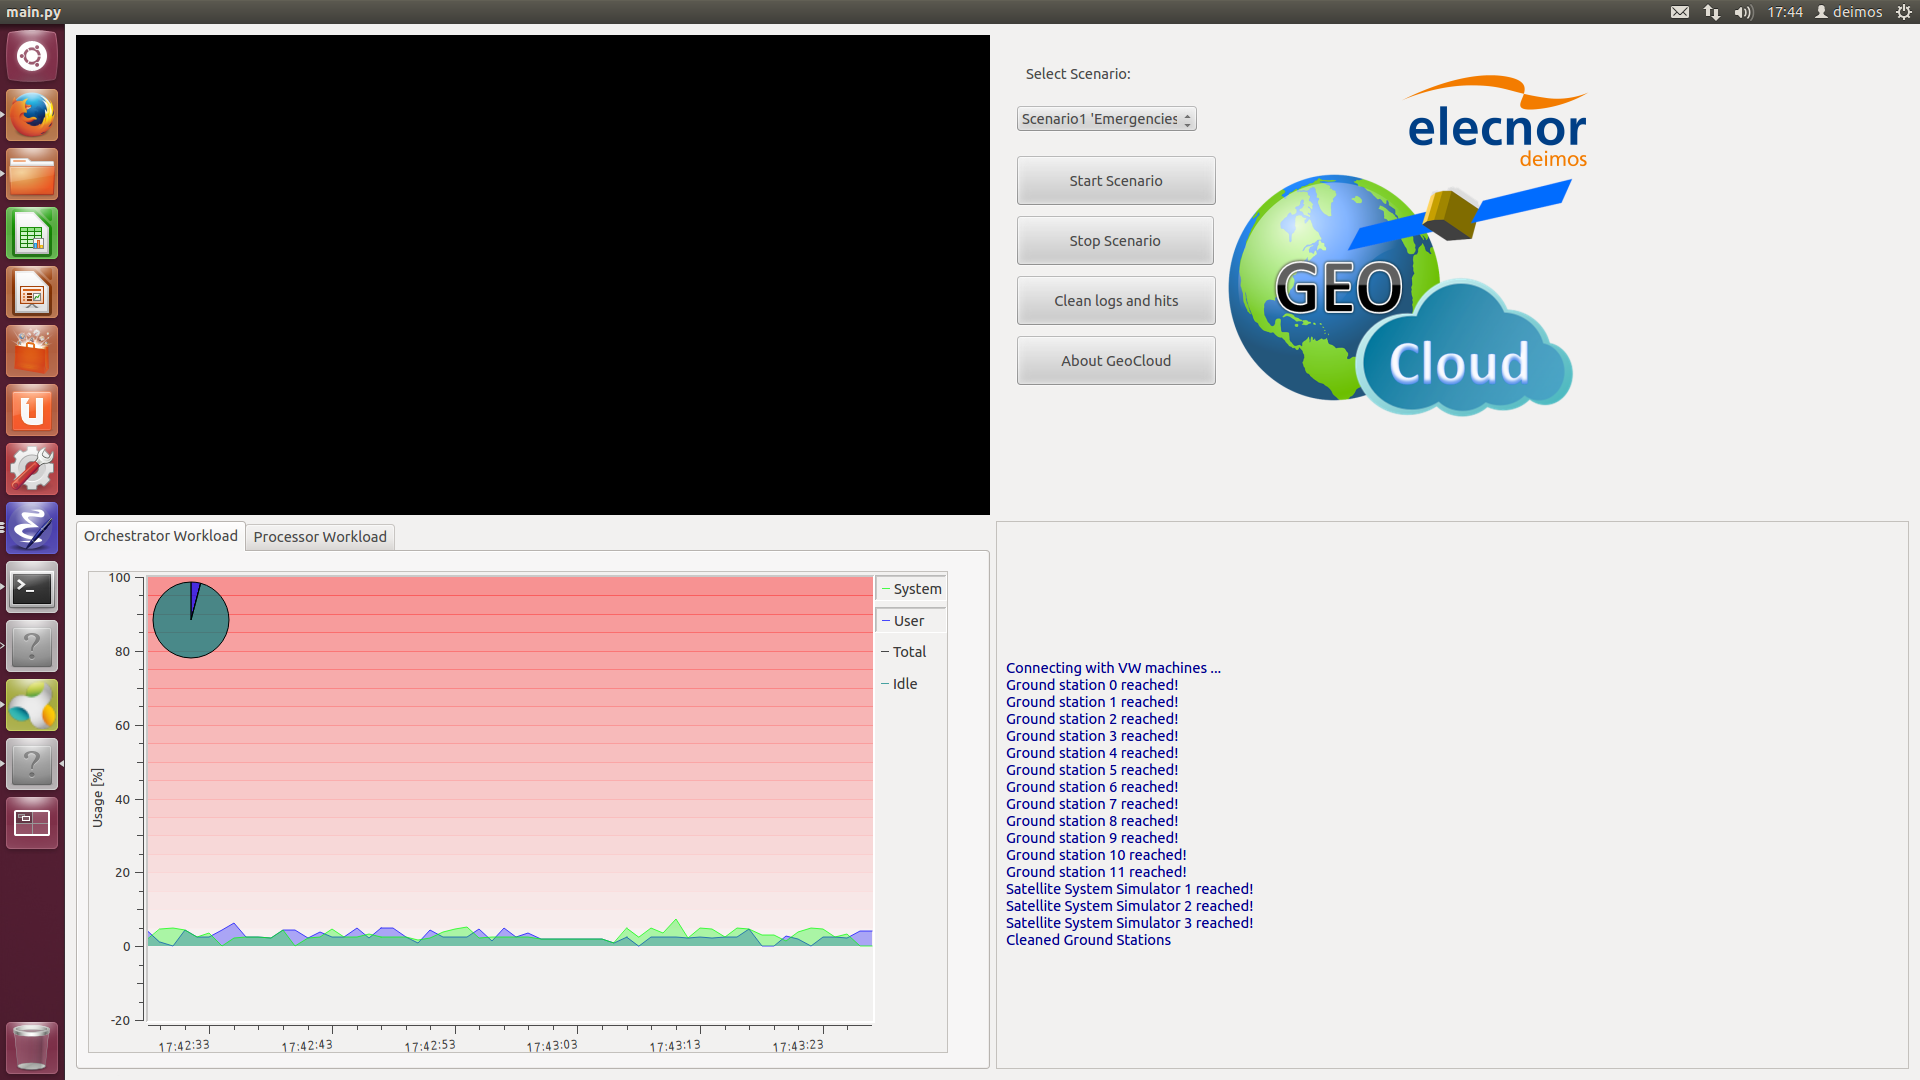
\includegraphics[width=1.1\textwidth]{gui/gui.png}
\caption{Components of the GUI}
\label{fig:gui-components}
\end{center}
\end{figure}



 





% Local Variables:
%   coding: utf-8
%   fill-column: 90
%   mode: flyspell
%   ispell-local-dictionary: "american"
%   mode: latex
%   TeX-master: "main"
% End:
